\papersubsection{Exception handling}


This section evaluates the performance of handling an exception from the host OS or hardware,
including installing an exception handler,
interrupting a running thread
with \palcall{ThreadInterrupt} (raising an \code{INTERRUPT} exception in the target thread),
and catching a hardware protection fault
(writing to a read-only address).






Figure~\ref{fig:eval:pal:sig-latency} (a)
shows the latency of installing an exception handler in either the Linux or \sgx{} PAL, compared with
\syscall{sigaction} in a Linux process.
The result
shows that regardless the PAL is running in a regular \picoproc{} or an enclave,
installing an exception handling
in the PAL
is much lower than install a signal handler
on Linux,
because the \hostapi{} does not have to take any system call or enclave exits.


Figure~\ref{fig:eval:pal:sig-latency} (b)
shows the latency of interrupting a running thread
and raising an exception
in the target thread, compared with delivering a \code{SIGUSR1} signal in a Linux process.
Thread interruption on the Linux PAL
is slightly slower than
delivering a \code{SIGUSR1} signal,
by \roughly{}25\% without \seccomp{} filter and reference monitor, or \roughly{}32\% with \seccomp{} filter and reference monitor.
On the \sgx{} PAL,
the latency of thread interrupt
is much higher, due to the cost of extra thread exits.
Interrupting a thread running on the \sgx{} PAL
is \roughly{}3.1$\times$ shower than delivering a \code{SIGUSR1} signal in a Linux process.



Figure~\ref{fig:eval:pal:sig-latency} (b)
shows the latency of catching a memory protection fault,
compared with handling
a \code{SIGSEGV} signal in a Linux process.
On the Linux, handling a hardware fault is \roughly{}2.6$\times$ slower than handling a \code{SIGSEGV} signal on Linux;
such an overhead
is primarily caused by delivering
the exception information to the guest, including the faulting register contexts.
Figure~\ref{fig:eval:pal:sig-latency} (b)
also shows that catching a hardware fault inside an enclave
is even more expensive
than thread interruption, by nearly 60\%.
The reason of such a dramatic difference is that
interrupting a thread only causes the interrupt thread to exit and enter the enclave once,
whereas handling a hardware fault
requires the faulting thread to exit and enter the enclave twice,
in order to reset the in-enclave buffer
for preserving the faulting contexts.


\begin{figure*}[t!]
\centering
\footnotesize
\resizebox{\textwidth}{!}{%
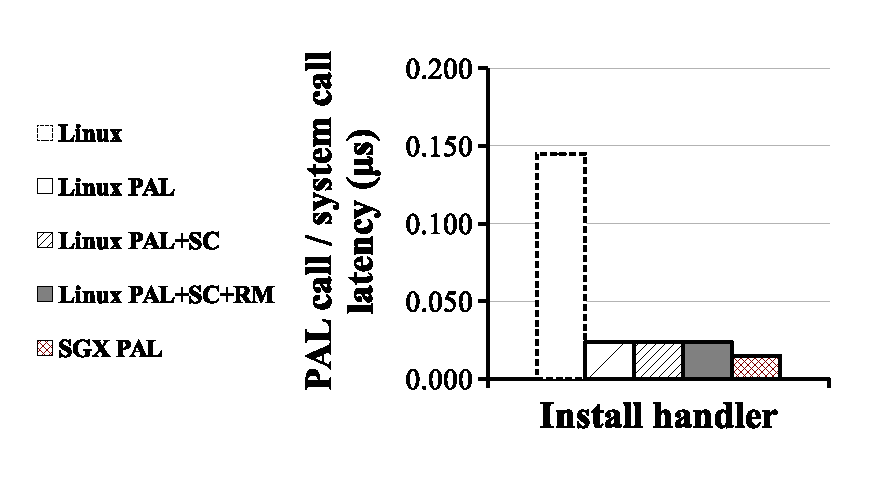
\includegraphics[height=10em]{sig-install-latency}
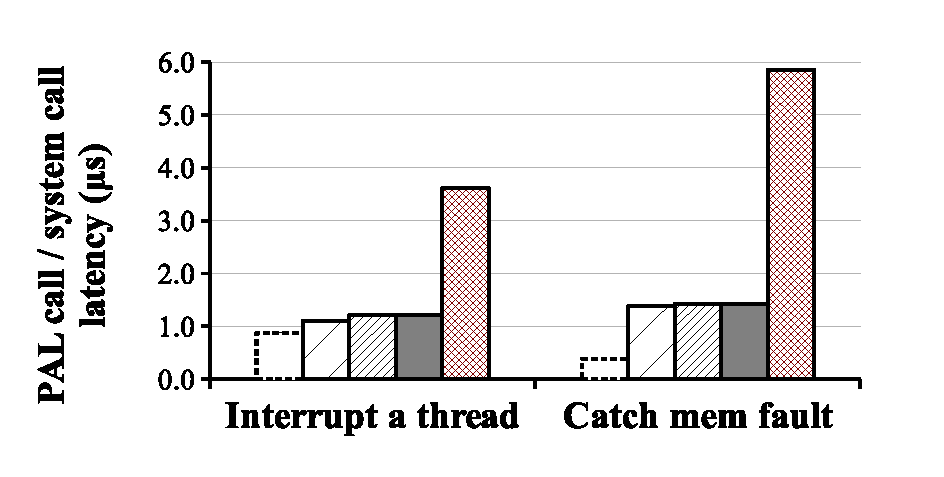
\includegraphics[height=10em]{sig-catch-latency}
}
\caption{Latency of (a) installing an exception handler; (b)
interrupting a running thread with signals (on Linux) or \palcall{ThreadInterrupt} on the PALs; (c) catching a memory protection fault. Lower is better. The comparison is between (1) signals on Linux; (2) the Linux PAL, with and without a \seccomp{} filter ({\bf +SC}) and reference monitor ({\bf +RM}); (3) the \sgx{} PAL.}
\label{fig:eval:pal:sig-latency}
\end{figure*}